\documentclass[11pt, a4paper, titlepage]{article}

% Set document dimensions
\usepackage[paper=a4paper,top=2cm,left=1.8cm,right=1.8cm,bottom=2cm, includefoot]{geometry}
\usepackage{float}
\usepackage[final]{pdfpages} % inludesvg

% Czech fonts
\usepackage[T1]{fontenc}
\usepackage[utf8]{inputenc}
\usepackage[czech]{babel}
\usepackage{fancyhdr}


\usepackage{background}
\setlength{\headheight}{3em} 
\newcommand{\subsectionbreak}{\clearpage}

\begin{document}
	\begin{titlepage}
    % \newgeometry{top=1in,top=2cm,left=2cm,right=2cm,bottom=2cm}

    \centering

    {\fontsize{20pt}{15pt}\bfseries
    VYSOKÉ UČENÍ TECHNICKÉ V~BRNĚ\\
    \vspace{8pt}
    Fakulta informačních technologií
    }


    
\includegraphics[scale=0.7]{./assets/fit-logo.pdf}

    \vspace{22pt}

    {\Large Přiručka k aplikaci do předmětu IVS\\}
    \vspace{40pt}
    {\Large \bfseries Super Science Calculator\\}
    
    \begin{figure}[h]
    \centering
    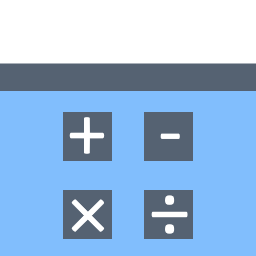
\includegraphics[scale=0.5]{./assets/icon.png}
    \end{figure}
    \vspace{10pt}
    {\Large \today}

    \vspace{90pt}
    {\Large \bfseries Autoři\\}
    \vspace{12pt}

    \begin{tabular}{ l c r }
        Martin Kobelka & \texttt{xkobel02} \\
        Karpíšek Jakub & \texttt{xkarpi06} \\
        Havlín Jan & \texttt{xhavli47} \\
        Vavro Ján & \texttt{xvavro05} \\
    \end{tabular}\\

\end{titlepage}
	\pagestyle{fancy}
	\lhead{\emph{Příručka k aplikaci do předmětu IVS}}
	\rhead{\emph{VUT FIT IVS 2017/2018}}
	\lfoot{\emph{VUT FIT - IVS}}
	\rfoot{\emph{Tým CodeIT@FIT}}

	\begin{center}
		\section*{Portfolio služeb}
	\end{center}

	\tableofcontents

	\section{Úvod}
	Následující dokument je uživatelskou příručkou k aplikaci super science calculator. Jedná se o projekt do
	předmětu IVS na FIT VUT vyučovaném v letním semestru akademického roku 2017/2018. kalkulačka nabízí 
	plnohodnotné matematické operace, systém proměnných včetně jejich závislostí a blokací smyček i základní podporu
	pro definování uživatelských funkcí.

	Aplikace je napsána v programovacích jazyích \texttt{Java} a \texttt{JavaSctript}. Je částečně pokryta jednotkovými testy.
	grafická vrstva aplikcace byla postavena ve frameworku \texttt{JavaFX}

	\section{Instalace}

\end{document}
